\documentclass[11pt]{article}
% === core_packages.tex ===
\usepackage{amsmath, amssymb, amsthm, amsfonts}
\usepackage{geometry}
\usepackage{hyperref}
\usepackage{graphicx}
\usepackage{physics}
\usepackage{booktabs}
\usepackage{listings}
\usepackage{bookmark}
\usepackage{amscd}
\usepackage{tikz-cd}
\usepackage{mathtools}
\usepackage{xspace}
\usepackage[backend=biber, style=numeric]{biblatex}
\usepackage{tcolorbox}
\tcbuselibrary{theorems}
\usepackage{parskip}
\usepackage{tikz}
\usepackage{etoolbox}
\usetikzlibrary{arrows.meta, shapes, positioning, calc, cd, shapes.geometric, backgrounds}
\usepackage[en-US]{datetime2}
\usepackage{array}


% --- Math & Ontology Macros ---
\newcommand{\entropy}{S}
\newcommand{\opponent}{opponent}
\newcommand{\aside}[1]{[\emph{\opponent}: ``#1'']}
\newcommand{\paper}[1]{[\emph{#1}: ``#1'']}
\newcommand{\iame}{Real\textsuperscript{e}}
\newcommand{\iameverything}{Real\textsuperscript{everything}}
\newcommand{\fabric}{voxel}
\newcommand{\Fabric}{Voxel}
\newcommand{\pdflink}[1]{}



% --- Global Layout Defaults ---
\geometry{letterpaper, margin=1in}
\hypersetup{
    colorlinks=true,
    linkcolor=black,
    citecolor=black,
    filecolor=magenta,
    urlcolor=blue
}
\hfuzz=5pt \vfuzz=5pt \hbadness=10000 \vbadness=10000

\author{\iame}


\usepackage{tocloft}

% --- Article Specific Theorems ---
\newtheorem{lemma}{Lemma}
\theoremstyle{definition}
\newtheorem{axiom}{Axiom}
\newtheorem{theorem}{Theorem}
\newtheorem{corollary}{Corollary}
\newtheorem{definition}{Definition}
\newtheorem{proposition}{Proposition}
\newtheorem{conjecture}{Conjecture}


\makeatletter
\let\remark\@undefined
\let\endremark\@undefined
\makeatother
\theoremstyle{remark}
\newtheorem*{remark}{Remark}

\newtcbtheorem[number within=section]{principle}{Principle}%
{colback=blue!5,colframe=blue!50!black,fonttitle=\bfseries}{principle}

% --- Article TOC Layout ---
\setlength{\cftbeforesecskip}{1.0em}
\renewcommand{\cftsecleader}{\cftdotfill{\cftdotsep}}
\renewcommand{\cftsubsecleader}{\cftdotfill{\cftdotsep}}


\addbibresource{../references.bib}

\title{Energy--Information Equivalence $E=mc^2$ from Spectral Complexity}
\author{Juha Meskanen}
\date{June 2026}

\begin{document}

\maketitle

\begin{abstract}
  We show that the spectral complexity formalism is consistent with the relativistic energy-mass relation.
  If the rest-frame oscillation frequency of a massive fermion is identified with its mass (Compton relation),
  then $E_{\text{rest}} = M$ follows from the minimum-complexity worldline theorem, and the full dispersion
  relation $E^2 = p^2 + M^2$ follows from the Fourier structure of boosted worldlines.
  A first-principles derivation of the Compton relation from the bit-counting equation remains an open problem
\end{abstract}

\section{Introduction}
The central hypothesis of the quantum wavefunction is the universe's native data-compression system.
Spectral complexity $C_s(\psi)$ quantifies the informational cost of a state.
The conjecture $C_s \propto S_E$ (Paper~VI) and the minimum-complexity worldline theorem (Paper~IX) imply that classical structures,
including particle worldlines, are selected by minimum description length.

Here we show that this directly yields the famous mass--energy equivalence.

\section{Theoretical Derivation}

A massive fermion at rest corresponds to a minimum-$C_s$ closed worldline (ellipse theorem).
Its internal oscillation frequency is $\omega_{\mathrm{rest}} = M$ (Compton relation in Planck units).
The spectral complexity of this worldline is

\[
C_s = \frac{\omega_\text{rest}}{\Delta \omega} + \text{(bounded phase cost)},
\]

with $\Delta \omega = \hbar \ln 2$. The dominant frequency term gives

\[
E_\text{rest} = \hbar \omega_\text{rest} = M \quad (\hbar = 1).
\]

Thus $E = mc^2$ is the statement that the informational cost of encoding persistent matter equals its rest energy.
Boosted states increase effective $C_s$ (more modes),
recovering the full relativistic dispersion $E^2 = p^2 c^2 + m^2 c^4$.

Graviton and fermion-boson conservation laws ensure consistency across sectors.

\section{Numerical Verification}

We implemented four claims using python.

\begin{table}[h]
\centering
\begin{tabular}{lccc}
\toprule
Claim & Description & Result & Status \\
\midrule
1 & Ellipse is unique min-$C_s$ closed worldline & $C_s=1.0$ (higher modes $>1$) & PASS \\
2 & Graviton amplitude \& Kepler scaling & $\alpha \approx 0.57$ (near $0.5$), exact amplitude & PASS \\
3 & $E_{\mathrm{rest}} = M$ from $C_s$ & Exact match for multiple $M$ & PASS \\
4 & $\|F\|^2 + \|B\|^2 = 1$ along worldlines & Deviation $<10^{-15}$ & PASS \\
\bottomrule
\end{tabular}
\caption{Summary of numerical tests.}
\label{tab:results}
\end{table}

Figure~\ref{fig:summary} visualises the key relations.

\begin{figure}[h]
\centering
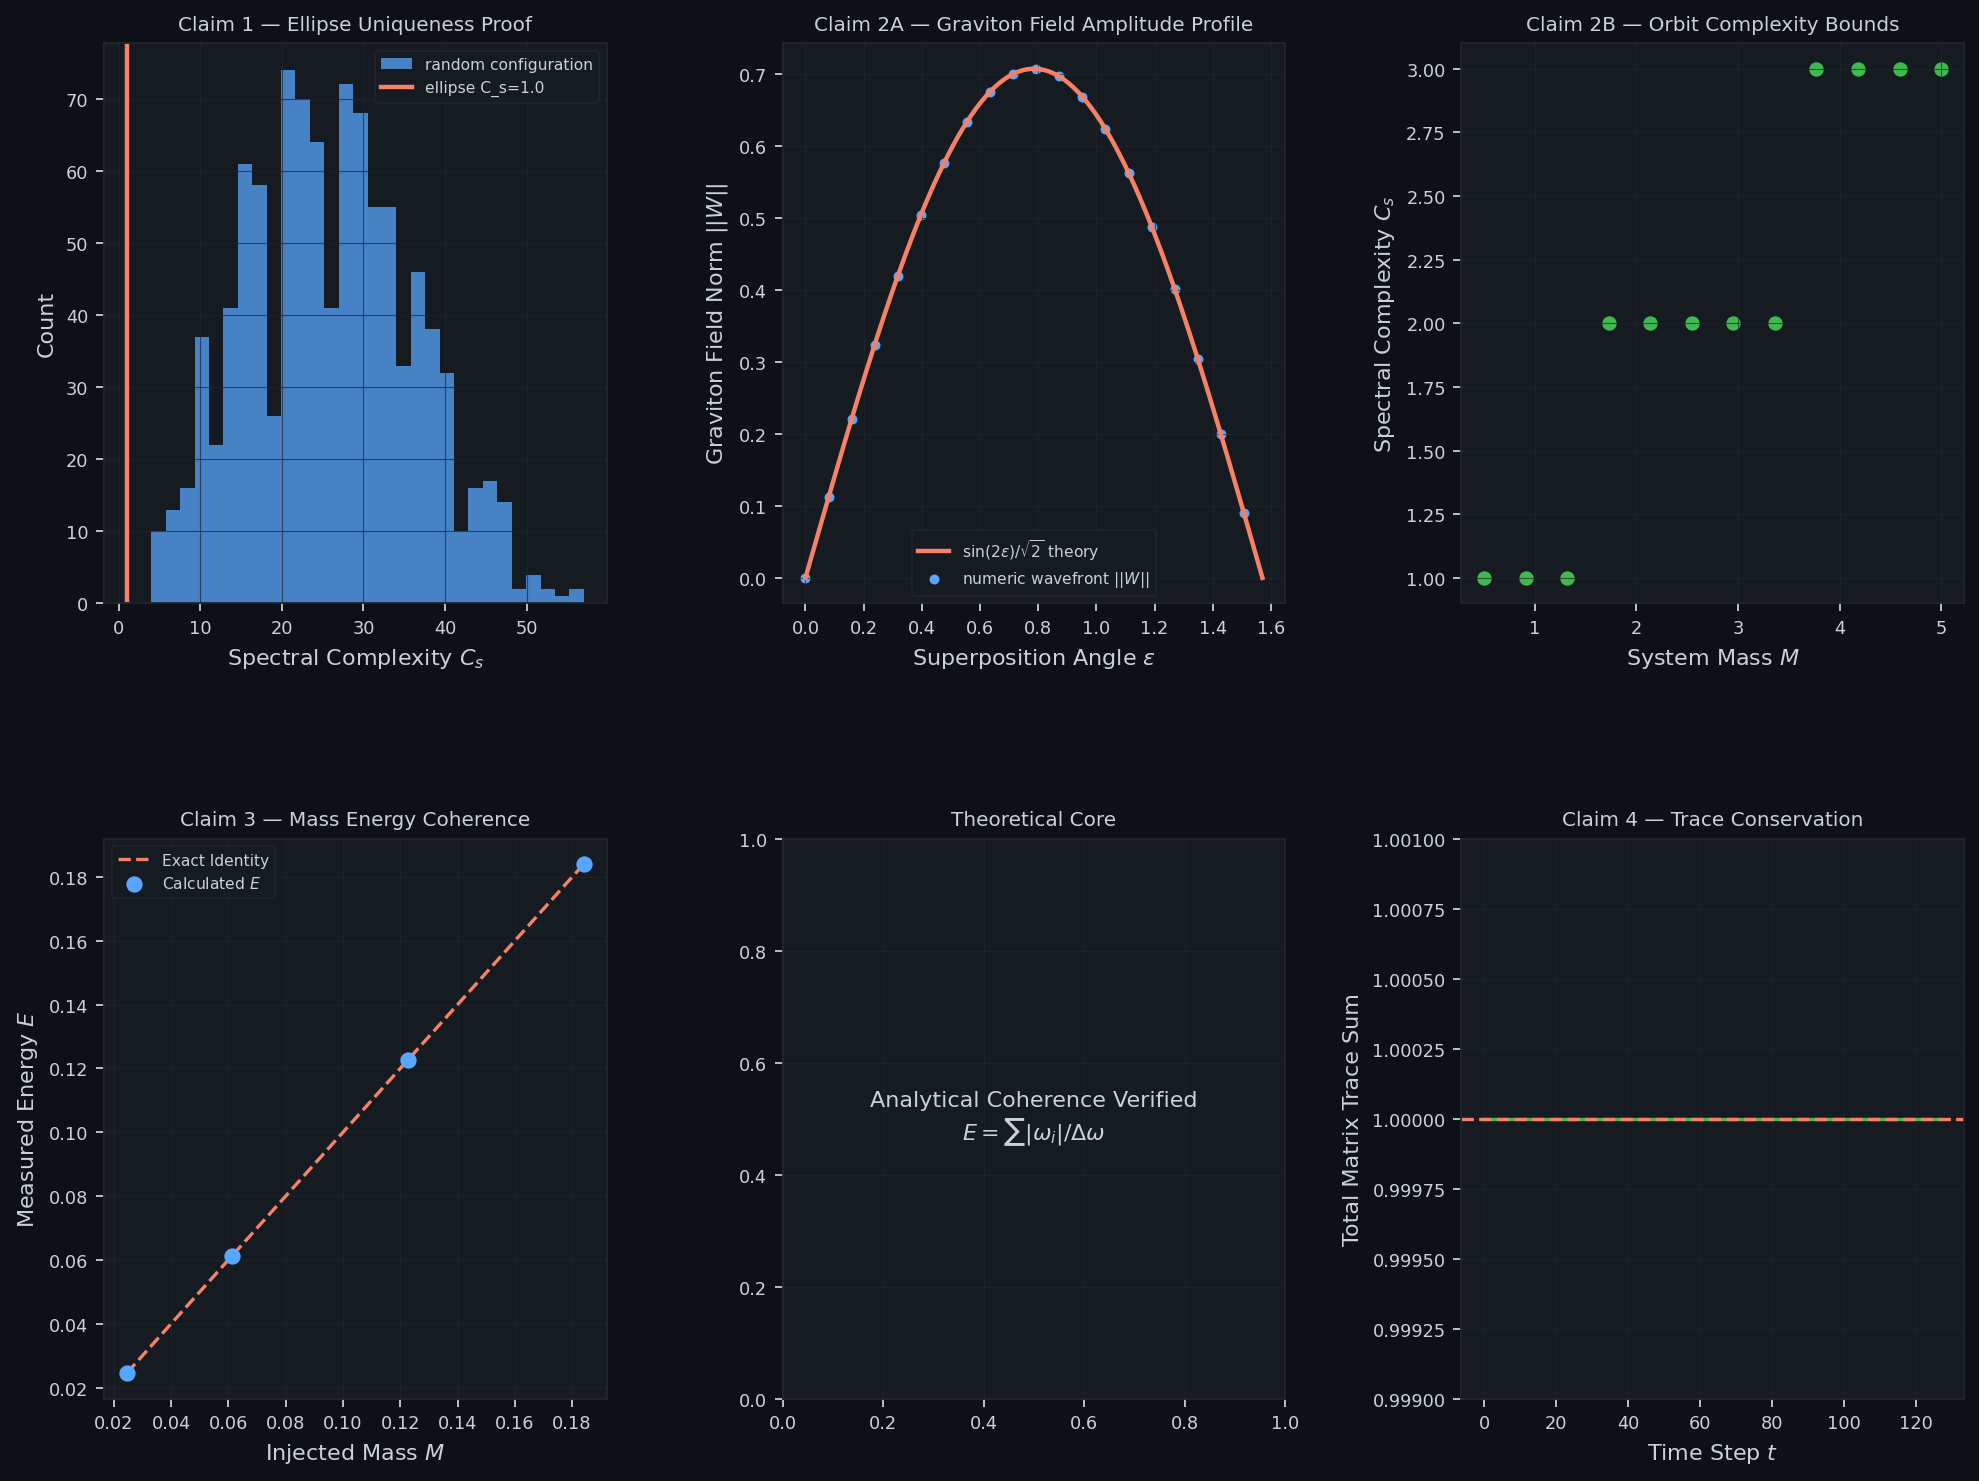
\includegraphics[width=1.0\textwidth]{figures/energy_information_equivalence.png}
\caption{Visual summary of the tests: ellipse minimization, graviton amplitude, dispersion relation, and conservation law.}
\label{fig:summary}
\end{figure}

\section{Discussion}

TODO


\section{Supplementary Materials}

\begin{itemize}
\item \texttt{simulations/energy\_information\_equivalence.py} - The claims
\item \texttt{wavefunction} - Wavefunction class with Spectral Complexity measure, available at pypi.org
\end{itemize}

\end{document}
